\documentclass[]{standalone}

\usepackage{amsmath}
\usepackage{amsfonts}
\usepackage{amssymb}
\usepackage{graphicx}
\usepackage{tikz}
\usepackage{import}
\usepackage{tikz_utils}
\usepackage[subpreambles=true]{standalone}

\usepackage{tikz}
\usepackage{tikz-3dplot}

\usetikzlibrary{positioning,decorations.markings, calc,math}

\begin{document}


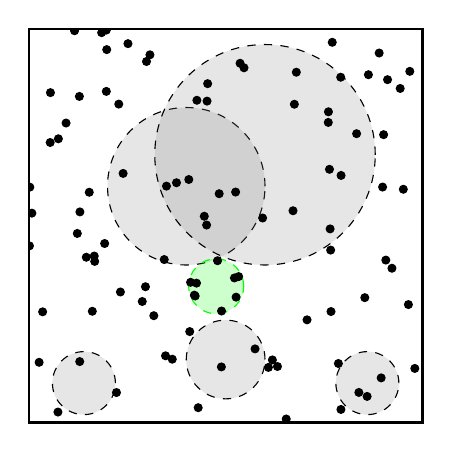
\begin{tikzpicture}[scale=1]

    \path[draw, thick] (0,0) rectangle (5,5);
    \clip (0,0) rectangle (5,5);
    \useasboundingbox (0,0) rectangle (5,5);
    \pgfmathsetmacro{\N}{100}
    \pgfmathsetseed{4}
    
    % dispersion circle
    \begin{scope}
        \clip (0,0) rectangle (5,5);
        \coordinate (center) at (2.805,3.62);
        \pgfmathsetmacro{\dispersion}{0.71};
        \path[draw, dashed, fill=gray, fill opacity=0.2] (0.7, 0.5) circle (0.4);
        \path[draw, dashed, fill=gray, fill opacity=0.2] (2,3) circle (1.0);
        \path[draw, dashed, fill=gray, fill opacity=0.2] (3,3.4) circle (1.4);
        \path[draw, dashed, fill=gray, fill opacity=0.2] (4.3,0.5) circle (0.4);
        \path[draw, dashed, fill=gray, fill opacity=0.2] (2.5, 0.8) circle (0.5);
        \path[draw=green, dashed, fill=green, fill opacity=0.2] (2.38, 1.73) circle (0.35);
    \end{scope}
    
    % draw the nodes
    \foreach \i in {1,...,\N} {
        \path[draw, fill] (rnd*5, rnd*5) circle (0.05);
    }
    


\end{tikzpicture}

\end{document}